\documentclass{tufte-handout}

\usepackage{amsmath}
\usepackage{tocbibind}

\usepackage{graphicx}
\setkeys{Gin}{width=\linewidth,totalheight=\textheight,keepaspectratio}
\graphicspath{{MyGraphics/}}

\title{Sound and Fourier Series: A Loving Relationship}
\author{Marshall Pangilinan}
\date{10 December 2015}

\usepackage{booktabs}

\usepackage{units}

\usepackage{fancyvrb}
\fvset{fontsize=\normalsize}

\usepackage{multicol}

\usepackage{lipsum}

\newcommand{\doccmd}[1]{\texttt{\textbackslash#1}}
\newcommand{\docopt}[1]{\ensuremath{\langle}\textrm{\textit{#1}}\ensuremath{\rangle}}
\newcommand{\docarg}[1]{\textrm{\textit{#1}}}
\newenvironment{docspec}{\begin{quote}\noindent}{\end{quote}}
\newcommand{\docenv}[1]{\textsf{#1}}% environment name
\newcommand{\docpkg}[1]{\texttt{#1}}% package name
\newcommand{\doccls}[1]{\texttt{#1}}% document class name
\newcommand{\docclsopt}[1]{\texttt{#1}}% document class option name

\begin{document}

\maketitle

\begin{abstract}
\noindent This paper provides a brief (and humorous) history and explanation of sound and Fourier series and shows the relationship between the two. As well, the Fourier series for the square wave is derived. This paper serves as an introductive guide to these two concepts.
\end{abstract}

\section{Sound}
\newthought{Sound has been around for a very long a time}. Maybe not as long as the universe, but certainly as long as there have been mediums for sound to travel in (ears, on the other hand, were completely unheard of until some few hundred million years ago \cite{Ear}). At an abstract level, sound is a disruption, or vibration, that travels through a medium, e.g. air or water, and transfers energy \cite{Harmony, Sound}. What we hear is a byproduct, similar to smell or taste or sight, our ability to hear is our brain's way of identifying and differentiating these vibrations. 

Sound travels in waves, but not just any waves! Sound travels in longitudinal waves! That is, the oscillations of the wave are parallel to the direction of the transfer of energy \cite{Sound}. This is very similar to the oscillation of a spring, consisting of compressions and rarefactions; the particles in the medium that sound travels through bounces off of itself, compresses, and stretches. This is also very similar to the oscillation of a long line of angry New Yorkers, where someone at the end of the line pushes the person in front of them, causing them to push the person in front of them before pushing back the original culprit and so on.

Sound can be represented graphically by sine and cosine functions of time, where the peaks and troughs of the function correlate to rarefactions and compressions respectively, and the zero is the equilibrium point.

	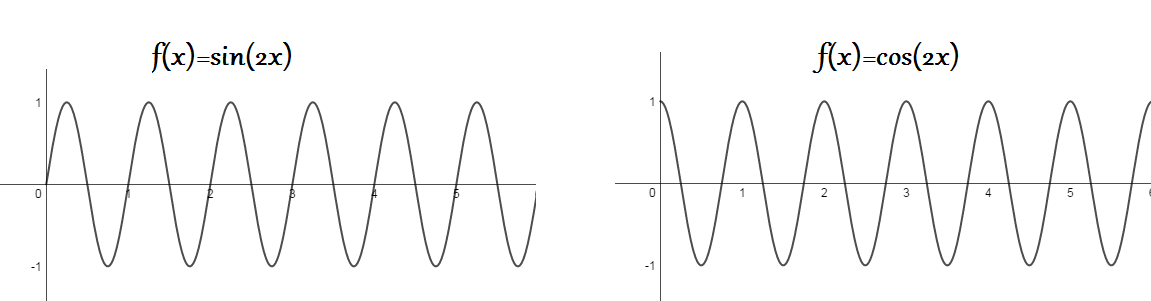
\includegraphics[width=\textwidth]{SinCos.png}

A sound wave has two important characteristics: amplitude, how far from the equilibrium point a particle oscillates; and frequency, how quickly, or frequently, those oscillations occur. We hear amplitude as volume, the greater the amplitude the louder the sound, and frequency as pitch, the higher the frequency the higher the pitch.

The speed of sound is very not constant. As stated earlier, sound needs a medium to travel; sound, unlike light, can not travel in a vacuum (although, vacuums cleaners are very loud). The speed of sound is wholly dependent on its medium; the speed of sound in dry air at 20 degrees Celsius is about 343 m/s \cite{Sound}. Sound travels faster in water because the particles in that medium are closer together. The line of angry New Yorkers is probably the slowest medium for sound to travel in.

An important quality of sound waves is when two or more waves interact with each other. Simply put, colliding sound waves will add together.

	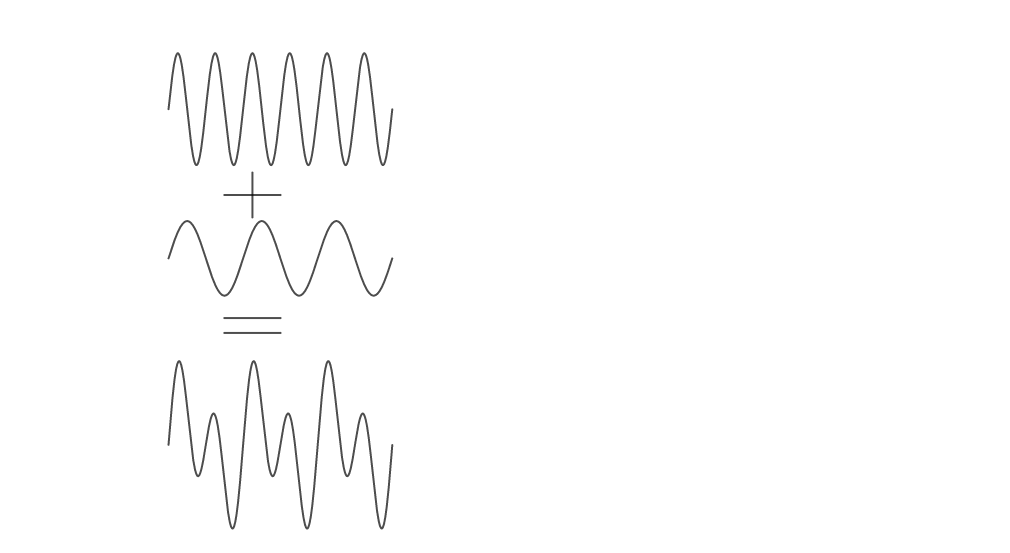
\includegraphics[width=8cm, height=5cm]{Collision.png}

	Resonance occurs when two sound waves of equal frequency add together and the amplitude increases; the compressions and rarefactions are happening at the same time and they compound each other.

	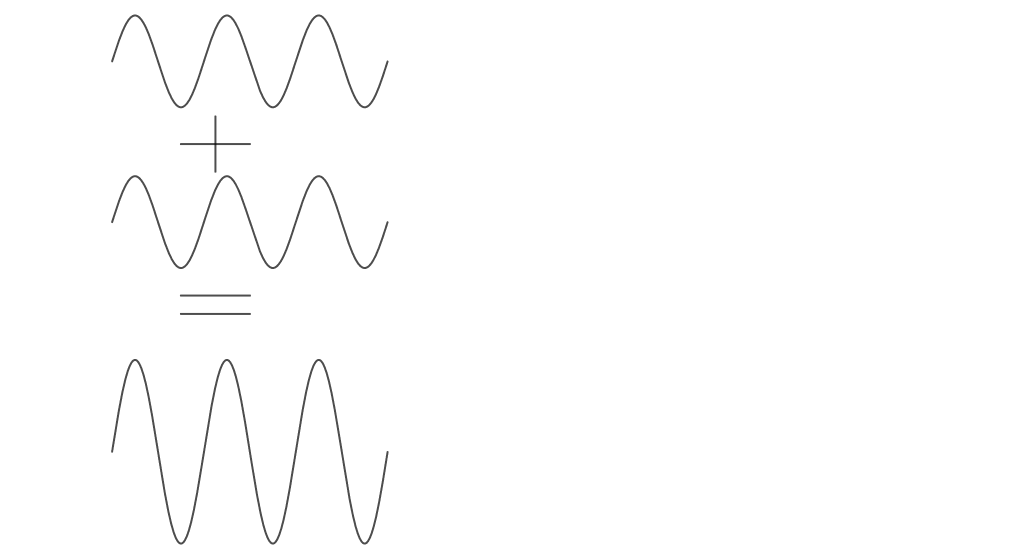
\includegraphics[width=8cm, height=5cm]{Resonance.png}

	Beats occur when two sound waves with frequencies that are close, but not equal, add together and the amplitude oscillates between audible and silent. The frequency of the beat is the difference between the frequencies of the sound waves.

	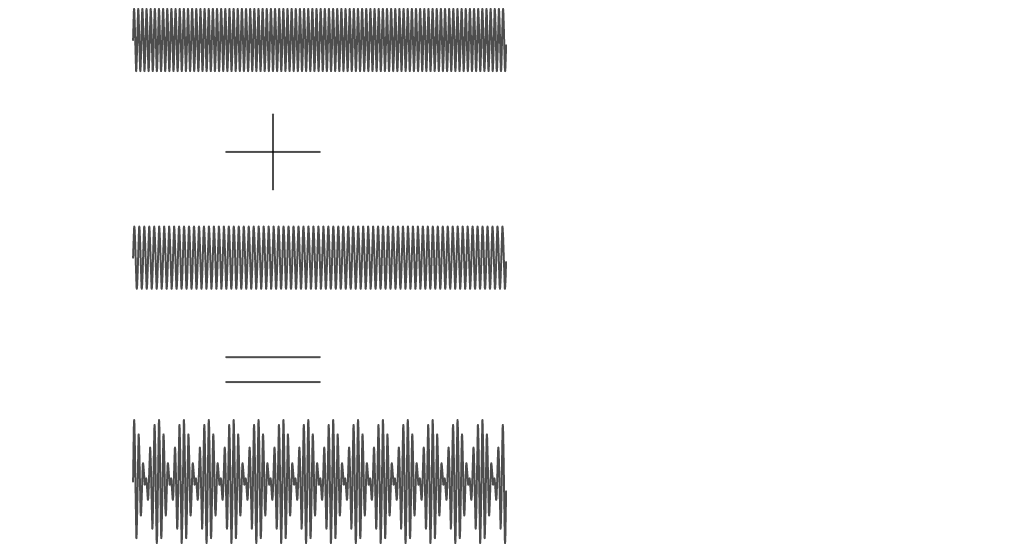
\includegraphics[width=8cm, height=5cm]{Beats.png}

Harmonics, or the wonderful pastime of blowing across the top of a root beer bottle, is a fascinating application of resonance. The reason a root beer bottle makes noise when blown into is because the air inside vibrates in such a way that it produces a sound that resonates with itself by reflecting off the bottom of the bottle. The frequency of this sound is the fundamental frequency, or the 1st harmonic \cite{Harmony}. There are three basic types of instruments that produce sound: strings, or where the medium of the sound is the object itself; open pipes, where air is the medium; and pipes closed at one end, where air is also the medium. The nature of each type of instrument affects the way a sound wave reflects and therefore affects the fundamental frequency.

The 2nd harmonic of an instrument is the second frequency that will resonate with itself, which happens to be twice the 1st harmonic. The 3rd harmonic is the third frequency that will resonate with itself, which happens to be thrice the 1st harmonic. The n-th harmonic is n multiplied by the fundamental frequency.

The fundamental frequency can be calculated if the speed of sound in that medium and the length of the instrument is known. For a string and an open pipe, the fundamental frequency completes half a wave before reflecting and resonating with itself. For a pipe closed at one end, the fundamental frequency completes a quarter of a wave. Knowing the velocity of sound in the medium, the fundamental frequencies can be calculated and represented as shown \cite{Harmony}:

For open pipes and strings of length L: $\newequation{f_1=\frac{v_sound}{2L}}$

For pipes closed at one end of length L: $\newequation{f_1=\frac{v_sound}{4L}}$

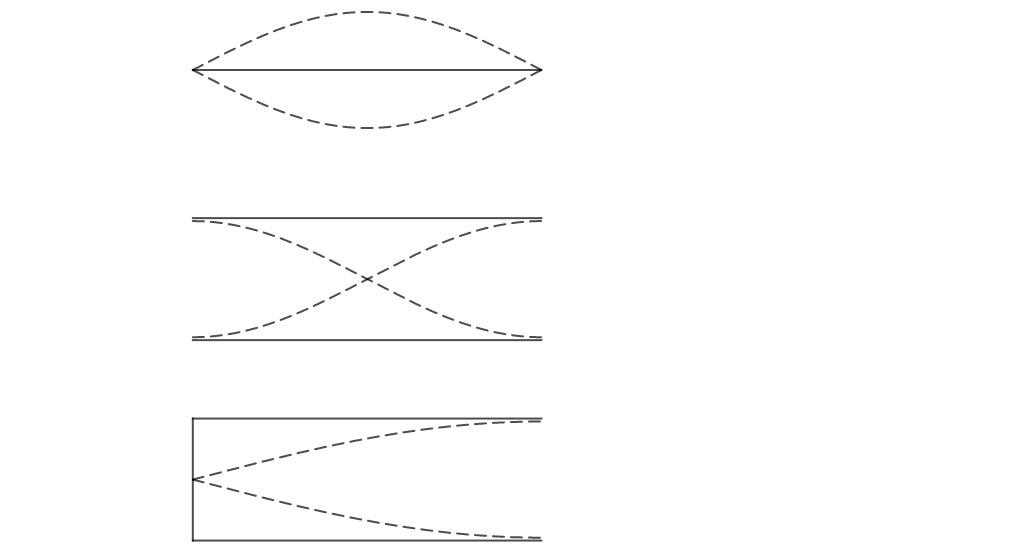
\includegraphics[width=8cm, height=5cm]{Harmonics.png}
	
	This sounds like a good stopping point for sounds for now.
\section{Fourier Series}
\newthought{A Fourier series}is a decomposition of a continuous, and usually periodic, function into the addition of an infinite amount of sines and cosines of varying amplitudes and frequencies. It is named after mathematician Jean-Baptiste Joseph Fourier (1768-1830), who introduced the series to solve the heat equation for a square plate \cite{FWho}. Fun fact! Way back when the Earth was the center of the universe circa 300 BCE (well after the birth of sound and the invention of ears), astronomists attempted to model the other planets' unusual paths around the Earth as epicycles, a series of circles orbiting around each other \cite{Earth}. This is similar to the addition of sines and cosines, functions defined by the unit circle (the radius of an orbit would be its amplitude and its orbital period would be the frequency); a common representation of a Fourier series are circles orbiting each other.

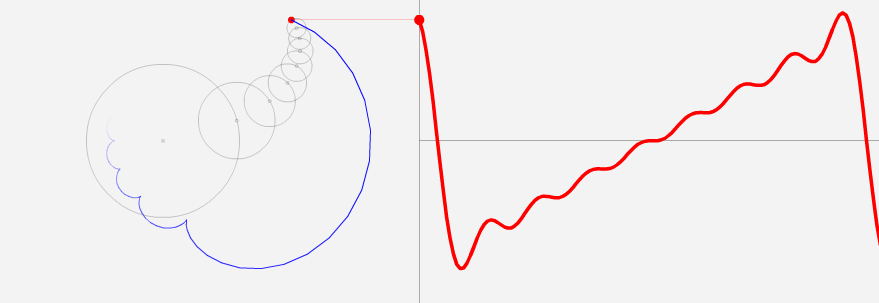
\includegraphics[width=8cm, height=5cm]{Circles.png}
	
Of course, literally any continuous path can be described by the addition of sines and cosines \cite{Homer}. A Fourier series can approximate any continuous function over a given period using the sum of sines and cosines, with increasing accuracy as the number of terms approaches infinity, especially if the function is periodic itself. 

The amplitude of each cosine and sine can be written as coefficients $a_n$ and $b_n$ respectively. The frequency of the waves can be written as $\frac{2\pi nx}{L}$. $\frac{2\pi}{L}$ is the fundamental frequency, and n is the n-th harmonic, just like the sound waves! But we'll get back to that later. The fourier series of a function f(x) over period L can be written as some constant $a_0$ and the summation of sines and cosines \cite{Wolfram, FWho}:
	
	\newequation{$$f(x)=a_0+\sum_{n=1}^{k}a_n\cos(\frac{2\pi nx}{L})+b_n\sin(\frac{2\pi nx}{L})$$}
	
Other inferior series, such as a Taylor series, require the function to also be differentiable. Fourier series scoffs at differentiability!
	
	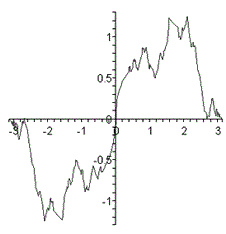
\includegraphics[width=8cm, height=5cm]{ScaryGraph.png}
	
Look at that! Sharp corners? I can't differentiate those! There's local extrema out the wazoo! But as long as the function is continuous, a Fourier series can approximate it. The problem is how to find the coefficients and frequencies of the summation.

The first step is to find the general coefficient of the general sine term, ${b_n}$. Note that the integral, or area under a graph, of a sine wave over at least one full period is 0. The peak and trough cancel each other out.

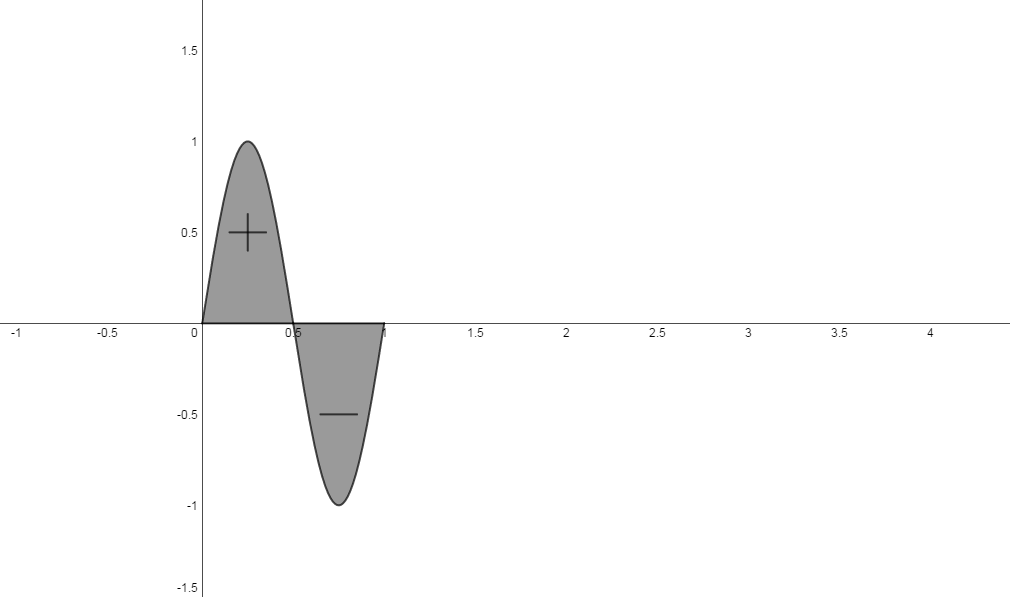
\includegraphics[width=8cm, height=5cm]{SinArea.png}

Consider the integral of the summation from 0 to L, where L is one full period of the funciton.
	\newequation{$$\int_0^L f(x)dx=\int_0^L a_0+\sum_{n=1}^{\infty}a_n\cos(\frac{2\pi nx}{L})+b_n\sin(\frac{2\pi nx}{L})dx$$}
Note that when a sine function is multiplied by a cosine function the result is a trig identity for a sine function, whose integral over at least one full period is 0. Therefore, all the cosine terms in the summation will cancel out. Similarly, multiplying two sine functions will result in symmetrical peaks and troughs that cancel each other out when integrated unless (and this is a big unless) the frequencies of the sine waves are equal; this will result in a square sine function, which has a positive area. Therefore, the n-th term can be isolated by multiplying both sides of the integral by ${\sin(\frac{2\pi nx}{L})}$.
	
	\newequation{$$\int_0^L f(x)\sin(\frac{2\pi nx}{L})dx=\int_0^L b_n\sin^2(\frac{2\pi nx}{L})dx$$}

The right side of this simplified equation can now be integrated.
	
	\newequation{$$\int_0^L b_n\sin^2(\frac{2\pi nx}{L})dx$$
	$$b_n\int_0^L \frac{1-\cos(\frac{2*2\pi nx}{L})}{2}dx$$
	$$b_n[\frac{x}{2}-\frac{L\sin(\frac{4\pi nx}{L})}{8\pi}]_0^L$$
	$$b_n[(\frac{L}{2}-0)-(0-0)]$$
	$$b_n\frac{L}{2}$$}

And therefore
	
	\newequation{$$\int_0^L f(x)\sin(\frac{2\pi nx}{L})dx=b_n\frac{L}{2}$$
	$$b_n=\frac{2}{L}\int_0^L f(x)\sin(\frac{2\pi nx}{L})dx$$}

The same process can be repeated for the cosine terms, resulting in the following equation:

	\newequation{$$a_n=\frac{2}{L}\int_0^L f(x)\cos(\frac{2\pi nx}{L})dx$$}

Success! We now have a way to find the coefficient for any term of the Fourier series for a given function!

\section{Fourier Series and Sound}
\newthought{Fourier series and Sound are very similar}. Sound travels in waves that can be represented by sine and cosine functions, with fundamental frequencies and n-th harmonics. Fourier series is a summation of sines and cosines also with fundamental frequencies and n-th harmonics! It's only logical that the two form a loving relationship, get married, and have a baby. What is that baby? Synthesising and approximating sounds. In fact, the ear is similar to a Fourier series. Inside the inner mechanisms of the ear are tiny hair follicles that resonate to different frequencies and, depending on which hairs are vibrating, the brain can interpret these resonating hairs as different sounds \cite{Ear}. If it's easier to comprehend, just believe that a tiny Fourier physicist lives inside the ear and tells the brain what's going on.

By recording a guitar, a voice, or some other audio, and performing Fourier analysis on the waveform, a synthesis, or synth, of that sound is created. The synth can be as accurate as desired by increasing the number of terms in the Fourier series. That synth can then be altered in various ways to produce new sounds which can be heard from a speaker. A speaker, which basically just oscillates back and forth, is like Fourier series machine.
	
Fourier series can also be used to approximate unusual sound waves. Back in the day of classic video games such as Super Mario Brothers (well after the birth of sound, the invention of ears, and the Earth's resignation from the center of the universe), music and sound effects were mostly described as triangle waves, sawtooth waves, and square waves \cite{Wolfram, Chip}.

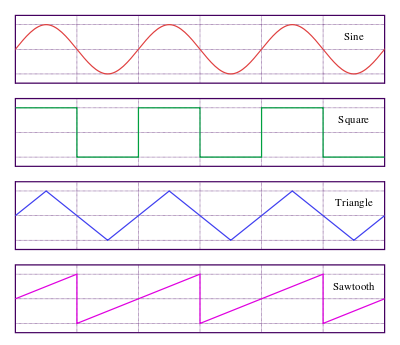
\includegraphics[width=8cm, height=5cm]{Waveforms.png}

But these waves are unusual; there are sharp corners, instant changes in position, it's bananas! As explained earlier, Fourier series does not care about these oddities.
	
Let's take a look at the square wave, aptly named because it didn't show up to the party last night and because of the rectangular shape of its graph. It is a simple binary wave: there are only two extreme positions, complete rarefaction and complete compression. Let's set some dimensions to ease the Fourier analysis. The first half of the wave can be described by the function

\newequation
$${f(x)=1 \{0\leq x\leq 1\}}$$

The second half can likewise be described by the function

\newequation
$${f(x)=-1 \{1\leq x\leq 2\}}$$

The square wave is now set with some easy-to-work-with numbers; the peaks and troughs are 1 and -1 respectively and the period is 2, which simplifies the general frequency of ${2\pi n/L}$ to ${\pi n}$ Fourier analysis can be performed on each half separately to added back together to find the general coefficient which can be used to define a new summation. Since this is an odd function, it has the property \newequation{-f(x)=f(-x)}, there will be no cosine terms.

	Step 1: Set up integral
	
	\newequation$${b_n=\int_0^1 \sin(\pi nx)dx}$$
	
	Step 2: Integrate!
	
	\newequation$${b_n=[\ \frac{-\cos(\pi nx)}{\pi n}]_0^1\ $$ 
	
	$$b_n=(\frac{-\cos(\pi n)}{\pi n})-(\frac{-\cos(\pi n0)}{\pi n})}$$

    Step 3: Analyze and simplify! {$\newequation{-\cos(\pi n)}$} will either be 1 when n is even or -1 when n is odd. {$\newequation{-\cos(\pi n0)}$} is always -1 regardless of the value of n.
    
    \newequation$${b_n=\frac{(-1)^{n+1}+1}{\pi n}}$$
    
    Step 3.5: Analyze and simplify more! The above equation will always be 0 when n is even and ${2/(\pi n)}$ when n is odd. So it can be rewritten by replacing n with 2n-1.
    
    \newequation$${b_n=\frac{2}{2\pi n-\pi}}$$
    
    Step 4: Repeat steps 1-3.5 with the second half of the function.
    
    \newequation$${b_n=\int_1^2 -\sin(\pi nx)dx$$
    
   $$ b_n=[\ \frac{\cos(\pi nx)}{\pi n}]_1^2\ $$
    
   $$ b_n=(\frac{\cos(2\pi n)}{\pi n})-(\frac{\cos(\pi n)}{\pi n})$$
    
    $$b_n=\frac{1+(-1)^{n+1}}{\pi n}$$
    
    $$b_n=\frac{2}{2\pi n-\pi}}$$

    Now that both halves of the general coefficient have been derived, they can be added together and substituted back into the original summation. Below is the Fourier series for the square wave and the graphs of k=[1,2,5,10,50]. Notice that as k increases the Fourier series approaches the original square wave graph.
    
    \newequation{$$f(x)=\sum_{n=1}^{k} \frac{4\sin(2\pi nx-\pi x)}{2\pi n-\pi}$$}
    
    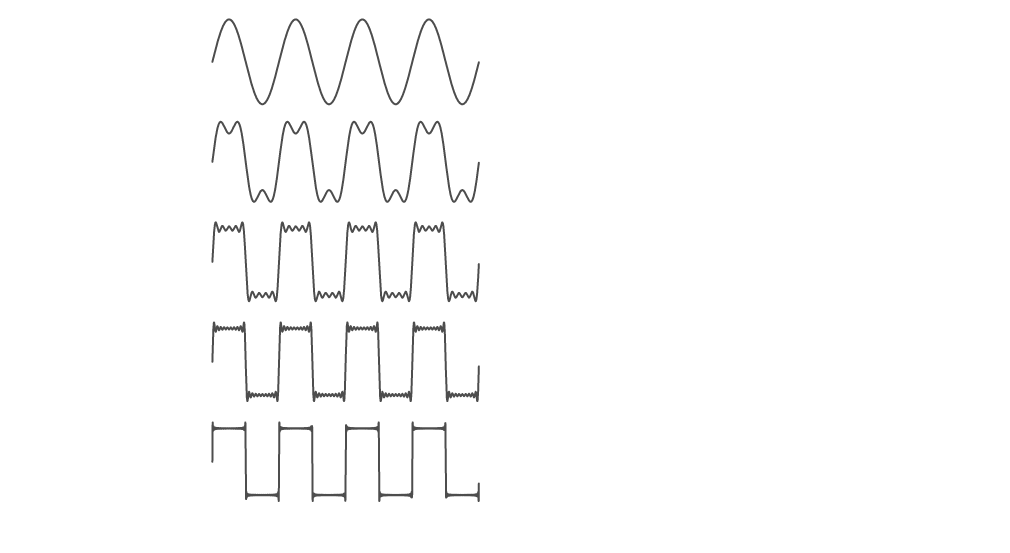
\includegraphics[width=8cm, height=5cm]{FourierSquare.png}
    
The sound quality of a square wave has a slight buzz to it, which is clearly shown from the Fourier series to be all (or almost all) of the odd harmonics. The fundamental frequency is still the dominating pitch, as it has the greatest amplitude. In fact, as the frequency of a square wave rises it becomes increasingly indiscernible from a regular sine wave, because at some point the next harmonic in the Fourier series is too high a frequency for human ears to detect \cite{Buzz}.

With your new found knowledge of sound, Fourier series, and angry New Yorkers, you can begin to analyze complex sound waves and derive your own Fourier series!

\bibliography{Refer.bib}
\bibliographystyle{unsrt}



\end{document}
